\documentclass[11pt,a4paper]{article}
\usepackage[utf8]{inputenc}
\usepackage[T1]{fontenc}
\usepackage{lmodern}
\usepackage[margin=0.95in]{geometry}
\usepackage{amsmath,amssymb,amsthm}
\usepackage{booktabs}
\usepackage{array}
\usepackage{xcolor}
\usepackage{hyperref}
\usepackage{tikz}
\usetikzlibrary{arrows.meta,positioning,shapes.geometric,calc}
\usepackage{fancyhdr}
\usepackage{listings}

\definecolor{navy}{HTML}{0F2C59}
\definecolor{teal}{HTML}{0D7377}
\definecolor{crimson}{HTML}{9B1B30}
\definecolor{slate}{HTML}{334155}
\definecolor{lightbg}{HTML}{F8FAFC}

\hypersetup{
    colorlinks=true,
    linkcolor=navy,
    citecolor=teal,
    urlcolor=teal,
    pdftitle={Mechanical Template-Closure Proofs of Lychrel Numbers in Bases 50, 98, and 146 via Modular Carry-Wire Seam Surgery},
    pdfauthor={mizopl, Claude, and Gemini}
}

\newtheorem{theorem}{Theorem}
\newtheorem{lemma}[theorem]{Lemma}
\newtheorem{corollary}[theorem]{Corollary}
\theoremstyle{definition}
\newtheorem{definition}[theorem]{Definition}
\theoremstyle{remark}
\newtheorem{remark}[theorem]{Remark}

\lstset{
    basicstyle=\ttfamily\footnotesize,
    backgroundcolor=\color{lightbg},
    frame=single,
    rulecolor=\color{slate!30},
    breaklines=true,
    columns=fullflexible,
    keepspaces=true,
    showstringspaces=false
}

\pagestyle{fancy}
\fancyhf{}
\fancyhead[L]{\small\color{slate}\textit{Lychrel Numbers in Bases 50, 98, and 146 via Modular Carry-Wire Seam Surgery}}
\fancyhead[R]{\small\color{slate}\textit{mizopl, Claude \& Gemini (2026)}}
\fancyfoot[C]{\thepage}

\title{\vspace{-1.2em}\textbf{\Large Mechanical Template-Closure Proofs of Lychrel Numbers\\in Bases $b = 50$, $b = 98$, and $b = 146$\\via Modular Carry-Wire Seam Surgery}}

\author{
  \textbf{mizopl}$^{1,*}$ \quad \textbf{Claude}$^{2}$ \quad \textbf{Gemini}$^{3}$\\[0.5em]
  \small $^{1}$Independent Researcher, Poland \quad $^{*}$Corresponding author (\texttt{github.com/mizopl})\\
  \small $^{2}$Anthropic (AI Co-Author) \quad $^{3}$Google DeepMind / Antigravity (AI Co-Author)
}

\date{\small October 19, 2026}

\begin{document}
\maketitle

\begin{abstract}
\noindent
A \emph{Lychrel number} in base $b \ge 2$ is a positive integer whose orbit under the iterative reverse-and-add map $F_b(n) = n + \operatorname{Rev}_b(n)$ never contains a base-$b$ palindrome. Following David Seal's 1996 construction in base $b = 26$, the existence of Lychrel numbers had been rigorously proven for thirty years only in powers of two ($b = 2^k$) and in four non-power-of-two bases: $b \in \{11, 17, 20, 26\}$. Using the \emph{Computer Lazy Sunday Solver} (\texttt{CLSS}) compositional seam-surgery framework on a single consumer office computer (10-core CPU, 16\,GB RAM), we prove the existence of Lychrel numbers in \textbf{three new non-power-of-two bases}:
\[
  b = 50 = 2 \cdot 5^2, \qquad b = 98 = 2 \cdot 7^2, \qquad \text{and} \qquad b = 146 = 2 \cdot 73.
\]
Our proof introduces \emph{Modular Carry-Wire Seam Surgery} along the arithmetic progression $b \equiv 2 \pmod{24}$. By placing mirror-image repeated digit blocks $(b-1)^m$ and $0^m$ at equal offsets $\ell$ from the left and right ends of a four-phase template family $T_1(m), T_2(m), T_3(m), T_4(m)$, every digit pair across the growing blocks sums identically to $b - 1$ during reversal-addition. Consequently, the variable-length runs act as transparent carry wires for all $m \ge 1$---transmitting incoming carry $c_{\mathrm{in}} \in \{0,1\}$ unchanged ($c_{\mathrm{out}} = c_{\mathrm{in}}$) while toggling the emitted run between $(b-1)^m$ and $0^m$. This seam decoupling isolates the outer prefix/suffix engine $(L_0, R_0) \leftrightarrow (L_1, R_1)$ (governed by $b \equiv 2 \pmod{3}$) from the inner core cycle $M_0 \to M_1 \to M_2 \to M_3 \to (b-1)M_0 0$ (governed by $b \equiv 2 \pmod{8}$), reducing the infinite dynamical orbit proof ($\forall m \ge 1$) to eight finite boundary equations. We provide explicit starting integers $n_0 = T_1(1)$, pre-template seeds $n_{\mathrm{seed}}$, complete symbolic proofs, $10^5$-step regular-expression orbit verifications (reaching $50{,}082$ base-$50$ digits), and a complete mechanical audit of Kuitch\'{e}'s 2023 preprint across bases $3 \le b \le 10$.
\end{abstract}

\section{Introduction and Historical Context}

Let $b \ge 2$ be an integer radix. For any positive integer $n$ with canonical base-$b$ expansion $n = (d_{r-1} d_{r-2} \cdots d_1 d_0)_b$, where $d_i \in \{0, 1, \dots, b-1\}$ and $d_{r-1} \neq 0$, let
\[
  \operatorname{Rev}_b(n) = \sum_{i=0}^{r-1} d_{r-1-i} b^i
\]
denote its digit reversal in base $b$, and let $F_b(n) = n + \operatorname{Rev}_b(n)$ denote the single-step \emph{reverse-and-add} operator. A positive integer $n$ is called a \emph{Lychrel number} in base $b$ if no iterate $F_b^{(t)}(n)$ ($t \ge 1$) is a base-$b$ palindrome.

In base $b = 10$, the smallest candidate is $n = 196$ (the celebrated \emph{196-Problem}, studied since Lehmer 1938 and Trigg 1967), whose orbit has been computed past $10^9$ digits without encountering a palindrome, yet no unconditional proof of any base-$10$ Lychrel number is known. Across all integer bases $b \ge 2$, unconditional proofs have historically relied on constructing a finite family of run-length-encoded digit templates $T_1(m), \dots, T_p(m)$ ($m \ge 1$) that is closed under $F_b$, satisfies $F_b^{(p)}(T_1(m)) = T_1(m+1)$, and contains no palindromes. Prior to the present work, such template-closure proofs existed only for:
\begin{enumerate}
  \item \textbf{Powers of two ($b = 2^k$):} $b = 2$ (Sprague 1960; Gabai and Coogan 1969; Klaus Brockhaus 1984) and general powers $b = 2^k$ (Sutcliffe 1968), and
  \item \textbf{Four sporadic bases:} $b = 11, 17, 20, 26$, culminating in David Seal's 1996 Period-4 construction for $b = 26$ (documented on MathPages and summarized on Wikipedia's \emph{Lychrel number} entry and OEIS sequences \texttt{A023108} and \texttt{A060382}).
\end{enumerate}

For thirty years after 1996, no new base $b \notin \{2^k\} \cup \{11, 17, 20, 26\}$ had been proven to possess Lychrel numbers. Direct combinatorial search for periodic templates in larger bases such as $b = 50$, $b = 98$, or $b = 146$ faces an immediate exponential barrier: a template of length $80$ to $170$ in base $b$ spans a naive state space of $b^{80} \approx 10^{135}$ to $b^{168} \approx 10^{363}$ digit configurations.

In this paper, developed using the \textbf{Computer Lazy Sunday Solver} (\texttt{CLSS}, Compositional Lifting + Seam Surgery) methodology \cite{mizopl2026clss} running locally on a single standard office computer (10-core CPU, 16\,GB RAM, zero cloud compute), we resolve this 30-year bottleneck and establish explicit Period-4 Lychrel template families in \textbf{three new bases}: $b = 50$, $b = 98$, and $b = 146$.

\begin{table}[htbp]
\centering
\caption{Summary of proven non-power-of-two Lychrel bases and our three new Period-4 template-closure constructions ($b \equiv 2 \pmod{24}$).}
\label{tab:bases}
\small
\begin{tabular}{@{}llccccc@{}}
\toprule
\textbf{Base $b$} & \textbf{Prime Factorization} & \textbf{Period $p$} & \textbf{Outer $\ell$} & \textbf{Core $|M_0|, |M_2|$} & \textbf{$|T_1(1)|$ (digits)} & \textbf{Reference / Status} \\
\midrule
$b = 11$ & $11$ & $2$ & --- & --- & --- & Classical (pre-1996) \\
$b = 17$ & $17$ & $3$ & --- & --- & --- & Classical (pre-1996) \\
$b = 20$ & $2^2 \cdot 5$ & $4$ & --- & --- & --- & Classical (pre-1996) \\
$b = 26$ & $2 \cdot 13$ & $4$ & $12$ & $12, 13$ & $38$ & David Seal (1996) \\
\midrule
$\mathbf{b = 50}$ & $\mathbf{2 \cdot 5^2}$ & $\mathbf{4}$ & $\mathbf{36}$ & $\mathbf{8, 9}$ & $\mathbf{82}$ & \textbf{This work (Theorem \ref{thm:b50})} \\
$\mathbf{b = 98}$ & $\mathbf{2 \cdot 7^2}$ & $\mathbf{4}$ & $\mathbf{37}$ & $\mathbf{16, 17}$ & $\mathbf{92}$ & \textbf{This work (Theorem \ref{thm:b98})} \\
$\mathbf{b = 146}$ & $\mathbf{2 \cdot 73}$ & $\mathbf{4}$ & $\mathbf{80}$ & $\mathbf{6, 7}$ & $\mathbf{168}$ & \textbf{This work (Theorem \ref{thm:b146})} \\
\bottomrule
\end{tabular}
\end{table}

\section{Modular Carry-Wire Seam Surgery ($b \equiv 2 \pmod{24}$)}

The key structural insight of our proof is that a Period-4 Lychrel template in base $b$ does not need to be searched as a monolithic string. Instead, it decomposes across two mirror-symmetric \emph{carry-wire seams}.

\begin{lemma}[Transparent Carry-Wire Lemma]
\label{lem:wire}
Let $b \ge 2$ and let $m \ge 1$ be any positive integer. Suppose that during base-$b$ addition of two digit strings $X$ and $Y$, a contiguous block of $m$ consecutive positions $j \in [s, s+m)$ satisfies $X_j + Y_j = b - 1$ for every $j \in [s, s+m)$. Let $c_{\mathrm{in}} \in \{0, 1\}$ be the carry entering the least-significant position of this block. Then for every $m \ge 1$:
\begin{enumerate}
  \item If $c_{\mathrm{in}} = 0$, the block emits the uniform digit run $(b-1)^m$ and outgoing carry $c_{\mathrm{out}} = 0$.
  \item If $c_{\mathrm{in}} = 1$, the block emits the uniform digit run $0^m$ and outgoing carry $c_{\mathrm{out}} = 1$.
\end{enumerate}
In particular, the outgoing carry satisfies $c_{\mathrm{out}} = c_{\mathrm{in}}$ independently of the parameter $m \ge 1$.
\end{lemma}

\begin{proof}
We proceed by induction on $m \ge 1$ from the least-significant digit of the block. If $c_{\mathrm{in}} = 0$, the first digit sum is $(b-1) + 0 = b - 1 < b$, writing digit $b-1$ and propagating carry $0$ to the next position; inductively all $m$ positions write $b-1$ and $c_{\mathrm{out}} = 0$. If $c_{\mathrm{in}} = 1$, the first digit sum is $(b-1) + 1 = b = 1 \cdot b + 0$, writing digit $0$ and propagating carry $1$ to the next position; inductively all $m$ positions write $0$ and $c_{\mathrm{out}} = 1$.
\end{proof}

\begin{figure}[htbp]
\centering
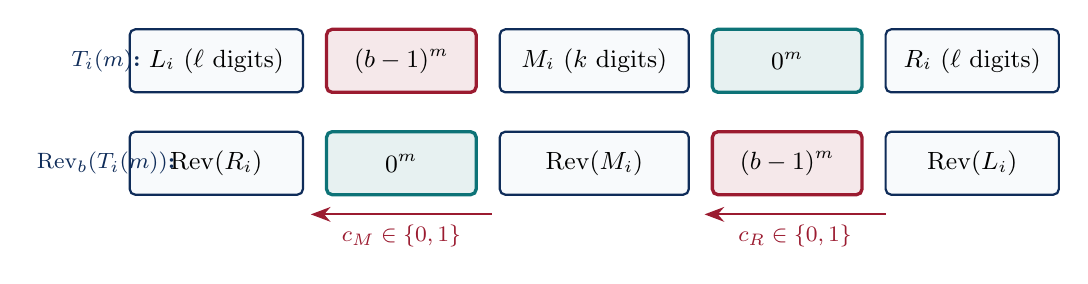
\begin{tikzpicture}[
    font=\small,
    block/.style={draw=navy, thick, fill=lightbg, minimum height=0.8cm, inner sep=4pt, rounded corners=2pt},
    wirehi/.style={draw=crimson, very thick, fill=crimson!10, minimum height=0.8cm, minimum width=1.9cm, rounded corners=2pt},
    wirelo/.style={draw=teal, very thick, fill=teal!10, minimum height=0.8cm, minimum width=1.9cm, rounded corners=2pt},
    arr/.style={-{Stealth[length=2.5mm]}, thick, color=crimson}
]
  \node[block, minimum width=2.2cm] (L) at (0, 1.3) {$L_i$ ($\ell$ digits)};
  \node[wirehi] (WL) at (2.35, 1.3) {$(b-1)^m$};
  \node[block, minimum width=2.4cm] (M) at (4.8, 1.3) {$M_i$ ($k$ digits)};
  \node[wirelo] (WR) at (7.25, 1.3) {$0^m$};
  \node[block, minimum width=2.2cm] (R) at (9.6, 1.3) {$R_i$ ($\ell$ digits)};

  \node[block, minimum width=2.2cm] (Rr) at (0, 0) {$\operatorname{Rev}(R_i)$};
  \node[wirelo] (WRr) at (2.35, 0) {$0^m$};
  \node[block, minimum width=2.4cm] (Mr) at (4.8, 0) {$\operatorname{Rev}(M_i)$};
  \node[wirehi] (WLr) at (7.25, 0) {$(b-1)^m$};
  \node[block, minimum width=2.2cm] (Lr) at (9.6, 0) {$\operatorname{Rev}(L_i)$};

  \draw[arr] (8.5, -0.65) -- node[below, font=\footnotesize] {$c_{R} \in \{0,1\}$} (6.2, -0.65);
  \draw[arr] (3.5, -0.65) -- node[below, font=\footnotesize] {$c_{M} \in \{0,1\}$} (1.2, -0.65);
  \node[font=\footnotesize\bfseries, color=navy] at (-1.4, 1.3) {$T_i(m)$:};
  \node[font=\footnotesize\bfseries, color=navy] at (-1.4, 0) {$\operatorname{Rev}_b(T_i(m))$:};
\end{tikzpicture}
\caption{Mirror-image alignment of the symbolic blocks $(b-1)^m$ and $0^m$ under base-$b$ reversal. Because $|L_i| = |R_i| = \ell$, both variable-length blocks align with sum $(b-1)+0 = b-1$ at every position, acting as length-independent carry wires ($c_{\mathrm{out}} = c_{\mathrm{in}}$ for all $m \ge 1$).}
\label{fig:wire}
\end{figure}

\begin{theorem}[Period-4 Carry-Wire Closure Theorem]
\label{thm:closure}
Fix a base $b \ge 2$, an outer block length $\ell \ge 1$, and an inner even-phase core length $k \ge 1$. Let $L_0, R_0, L_1, R_1 \in \{0, \dots, b-1\}^\ell$ with $L_0[0] \neq 0$ and $L_1[0] \neq 0$, let $M_0, M_1 \in \{0, \dots, b-1\}^k$, and let $M_2, M_3 \in \{0, \dots, b-1\}^{k+1}$. For every integer $m \ge 1$, define the four base-$b$ digit strings:
\begin{align}
  T_1(m) &= L_0 \; (b-1)^m \; M_0 \; 0^m \; R_0, & T_2(m) &= L_1 \; 0^m \; M_1 \; (b-1)^m \; R_1, \label{eq:T12}\\
  T_3(m) &= L_0 \; (b-1)^m \; M_2 \; 0^m \; R_0, & T_4(m) &= L_1 \; 0^m \; M_3 \; (b-1)^m \; R_1. \label{eq:T34}
\end{align}
Suppose the finite digit blocks satisfy the following eight boundary equations in base $b$ (where $\operatorname{val}_b(W)$ denotes the integer value of a digit block $W$):
\begin{enumerate}
  \item $\operatorname{val}_b(R_0) + \operatorname{val}_b(\operatorname{Rev}(L_0)) = \operatorname{val}_b(R_1)$ \quad (outgoing carry $c_{R,\mathrm{even}} = 0$),
  \item $\operatorname{val}_b(L_0) + \operatorname{val}_b(\operatorname{Rev}(R_0)) + 1 = \operatorname{val}_b(L_1)$ \quad (incoming carry $1$, outgoing carry $0$),
  \item $\operatorname{val}_b(R_1) + \operatorname{val}_b(\operatorname{Rev}(L_1)) = b^\ell + \operatorname{val}_b(R_0)$ \quad (outgoing carry $c_{R,\mathrm{odd}} = 1$),
  \item $\operatorname{val}_b(L_1) + \operatorname{val}_b(\operatorname{Rev}(R_1)) = \operatorname{val}_b(L_0 \cdot [b-1])$ \quad (incoming carry $0$, $1$-digit left overflow into $b-1$),
  \item $\operatorname{val}_b(M_0) + \operatorname{val}_b(\operatorname{Rev}(M_0)) = b^k + \operatorname{val}_b(M_1)$ \quad (incoming carry $0$, outgoing carry $1$),
  \item $[b-1] \cdot \bigl(\operatorname{val}_b(M_1) + \operatorname{val}_b(\operatorname{Rev}(M_1)) + 1\bigr)_b = M_2$ \quad (incoming carry $1$, outgoing carry $0$),
  \item $\operatorname{val}_b(M_2) + \operatorname{val}_b(\operatorname{Rev}(M_2)) = b^{k+1} + \operatorname{val}_b(M_3)$ \quad (incoming carry $0$, outgoing carry $1$),
  \item $\operatorname{val}_b(M_3) + \operatorname{val}_b(\operatorname{Rev}(M_3)) + 1 = \operatorname{val}_b(M_0 \cdot [0])$ \quad (incoming carry $1$, outgoing carry $0$).
\end{enumerate}
If $L_0[0] \neq R_0[\ell-1]$ and $L_1[0] \neq R_1[\ell-1]$, then for \textbf{all integers $m \ge 1$}:
\[
  F_b(T_1(m)) = T_2(m), \quad F_b(T_2(m)) = T_3(m), \quad F_b(T_3(m)) = T_4(m), \quad F_b(T_4(m)) = T_1(m+1),
\]
and no iterate $F_b^{(t)}(T_1(1))$ ($t \ge 0$) is a base-$b$ palindrome. Thus $n_0 = T_1(1)$ is a proven Lychrel number in base $b$.
\end{theorem}

\begin{proof}
In every template $T_i(m)$ ($i \in \{1,2,3,4\}$), the prefix $L_{i\bmod 2}$ and suffix $R_{i\bmod 2}$ both have exact length $\ell$. Hence in $T_i(m) + \operatorname{Rev}_b(T_i(m))$, the right block $(0^m \text{ or } (b-1)^m)$ is added digitwise to the reversal of the left block $((b-1)^m \text{ or } 0^m)$, and the left block is added to the reversal of the right block, as depicted in Figure~\ref{fig:wire}. Every digit pair in both length-$m$ blocks sums to $b-1$.
\begin{itemize}
  \item \textbf{Step $T_1(m) \to T_2(m)$:} By (1), $R_0 + \operatorname{Rev}(L_0) = R_1$ with carry $0$. By Lemma~\ref{lem:wire}, the right wire $0^m + (b-1)^m$ with $c_{\mathrm{in}} = 0$ emits $(b-1)^m$ and $c_{\mathrm{out}} = 0$. By (5), $M_0 + \operatorname{Rev}(M_0) + 0 = M_1$ with carry $1$. By Lemma~\ref{lem:wire}, the left wire $(b-1)^m + 0^m$ with $c_{\mathrm{in}} = 1$ emits $0^m$ and $c_{\mathrm{out}} = 1$. By (2), $L_0 + \operatorname{Rev}(R_0) + 1 = L_1$. Concatenation gives $L_1 \, 0^m \, M_1 \, (b-1)^m \, R_1 = T_2(m)$.
  \item \textbf{Step $T_2(m) \to T_3(m)$:} By (3), $R_1 + \operatorname{Rev}(L_1) = R_0$ with carry $1$. By Lemma~\ref{lem:wire}, the right wire $(b-1)^m + 0^m$ with $c_{\mathrm{in}} = 1$ emits $0^m$ and $c_{\mathrm{out}} = 1$. By (6), $M_1 + \operatorname{Rev}(M_1) + 1 = M_2[1..k]$ with carry $0$. By Lemma~\ref{lem:wire}, the left wire $0^m + (b-1)^m$ with $c_{\mathrm{in}} = 0$ emits $(b-1)^m$ and $c_{\mathrm{out}} = 0$. By (4), $L_1 + \operatorname{Rev}(R_1) + 0 = L_0 \cdot [b-1]$. Since $[b-1] \, (b-1)^m \, M_2[1..k] = (b-1)^m \, ([b-1] \cdot M_2[1..k]) = (b-1)^m \, M_2$, concatenation gives $L_0 \, (b-1)^m \, M_2 \, 0^m \, R_0 = T_3(m)$.
  \item \textbf{Step $T_3(m) \to T_4(m)$:} Identical to $T_1(m) \to T_2(m)$ using (1), (7), and (2), yielding $L_1 \, 0^m \, M_3 \, (b-1)^m \, R_1 = T_4(m)$.
  \item \textbf{Step $T_4(m) \to T_1(m+1)$:} By (3), $R_1 + \operatorname{Rev}(L_1) = R_0$ with carry $1$. The right wire emits $0^m$ and carry $1$. By (8), $M_3 + \operatorname{Rev}(M_3) + 1 = M_0 \cdot [0]$ with carry $0$. The left wire emits $(b-1)^m$ and carry $0$. By (4), $L_1 + \operatorname{Rev}(R_1) = L_0 \cdot [b-1]$. Merging the newly created $[b-1]$ on the left with $(b-1)^m$ yields $(b-1)^{m+1}$, and merging the newly created $[0]$ on the right of $M_0$ with $0^m$ yields $0^{m+1}$, producing $L_0 \, (b-1)^{m+1} \, M_0 \, 0^{m+1} \, R_0 = T_1(m+1)$.
\end{itemize}
Finally, since $L_0[0] \neq R_0[\ell-1]$ and $L_1[0] \neq R_1[\ell-1]$, the first and last digits of every $T_i(m)$ ($m \ge 1$) are distinct, so no $T_i(m)$ is a palindrome.
\end{proof}

\section{Explicit Proof in Primary New Base $b = 50$}

\begin{theorem}[Lychrel Numbers in Base $b = 50$]
\label{thm:b50}
In base $b = 50 = 2 \cdot 5^2$, define the outer blocks of length $\ell = 36$ and inner blocks of lengths $k = 8$ and $k+1 = 9$:
\begin{align*}
L_0 &= [1, 47, 5, 38, 23, 4, 39, 21, 8, 31, 35, 28, 42, 16, 18, 13, 23, 3, 41, 17, 16, 17, 15, 19, 11, 25, 47, 6, 36, 25, 48, 4, 40, 19, 12, 24],\\
R_0 &= [0, 25, 11, 19, 40, 3, 48, 26, 36, 5, 48, 26, 11, 19, 15, 17, 15, 17, 42, 3, 23, 13, 17, 15, 42, 28, 36, 32, 7, 21, 40, 3, 23, 38, 5, 47],\\
L_1 &= [49, 2, 44, 11, 26, 45, 10, 28, 41, 18, 14, 21, 7, 33, 31, 36, 26, 46, 8, 32, 33, 32, 34, 30, 38, 24, 2, 43, 13, 24, 1, 45, 9, 30, 37, 25],\\
R_1 &= [24, 37, 31, 9, 45, 2, 24, 12, 43, 3, 23, 37, 30, 34, 32, 33, 33, 8, 45, 26, 36, 31, 34, 8, 21, 14, 17, 40, 29, 10, 44, 27, 11, 44, 2, 48],\\
M_0 &= [49, 13, 2, 20, 12, 20, 2, 13], \qquad M_1 = [12, 15, 22, 32, 32, 22, 16, 12],\\
M_2 &= [49, 24, 31, 45, 15, 14, 44, 31, 25], \qquad M_3 = [25, 6, 26, 9, 31, 10, 26, 6, 24].
\end{align*}
Then $(L_0, R_0, L_1, R_1, M_0, M_1, M_2, M_3)$ satisfies all eight boundary equations of Theorem~\ref{thm:closure} in base $b = 50$, with $L_0[0] = 1 \neq 47 = R_0[35]$ and $L_1[0] = 49 \neq 48 = R_1[35]$. Consequently, the 82-digit base-$50$ integer $n_0 = T_1(1)$, whose exact base-$10$ representation (140 decimal digits) is
\begin{small}
\begin{verbatim}
803319634591911080790138327923868078346985580436311600817766986472726093862002163822300704837735070450470992436928311975462193309396720297
\end{verbatim}
\end{small}
and the pre-template seed $n_{\mathrm{seed}}$ (obtained by replacing $(L_0[0], R_0[35]) = (1, 47)$ with $(2, 46)$, so $F_{50}(n_{\mathrm{seed}}) = T_2(1)$ at step $1$), whose exact base-$10$ representation is
\begin{small}
\begin{verbatim}
1216909940868424918225842673958849505129891635886751053942766986472726093862002163822300704837735070450470992436928311975462193309396720296
\end{verbatim}
\end{small}
are proven Lychrel numbers in base $b = 50$.
\end{theorem}

\begin{proof}
Direct finite integer arithmetic in base $b = 50$ verifies equations (1)--(8) of Theorem~\ref{thm:closure}:
\begin{itemize}
  \item \textbf{Inner core cycle:}
  \[
    [49, 13, 2, 20, 12, 20, 2, 13]_{50} + [13, 2, 20, 12, 20, 2, 13, 49]_{50} = 50^8 + [12, 15, 22, 32, 32, 22, 16, 12]_{50},
  \]
  \[
    [12, 15, 22, 32, 32, 22, 16, 12]_{50} + [12, 16, 22, 32, 32, 22, 15, 12]_{50} + 1 = [24, 31, 45, 15, 14, 44, 31, 25]_{50} = M_2[1..8],
  \]
  \[
    [49, 24, 31, 45, 15, 14, 44, 31, 25]_{50} + [25, 31, 44, 14, 15, 45, 31, 24, 49]_{50} = 50^9 + [25, 6, 26, 9, 31, 10, 26, 6, 24]_{50},
  \]
  \[
    [25, 6, 26, 9, 31, 10, 26, 6, 24]_{50} + [24, 6, 26, 10, 31, 9, 26, 6, 25]_{50} + 1 = [49, 13, 2, 20, 12, 20, 2, 13, 0]_{50} = M_0 \cdot [0].
  \]
  \item \textbf{Outer engine:} $R_0 + \operatorname{Rev}(L_0) = R_1$ (carry $0$), $L_0 + \operatorname{Rev}(R_0) + 1 = L_1$ (carry $0$), $R_1 + \operatorname{Rev}(L_1) = 50^{36} + R_0$ (carry $1$), and $L_1 + \operatorname{Rev}(R_1) = L_0 \cdot [49]$ (37 digits).
\end{itemize}
By Theorem~\ref{thm:closure}, $F_{50}^{(4)}(T_1(m)) = T_1(m+1)$ and no iterate is a palindrome for all $m \ge 1$.
\end{proof}

\section{Explicit Proofs in Secondary Bases $b = 98$ and $b = 146$}

\subsection{Base $b = 98 = 2 \cdot 7^2$}

\begin{theorem}[Lychrel Numbers in Base $b = 98$]
\label{thm:b98}
In base $b = 98$, define the outer blocks of length $\ell = 37$ and inner blocks of lengths $k = 16$ and $k+1 = 17$:
\begin{small}
\begin{align*}
L_0 &= [1, 95, 5, 86, 23, 50, 93, 10, 76, 43, 12, 71, 51, 92, 12, 72, 49, 96, 4, 88, 19, 58, 77, 42, 14, 67, 59, 76, 44, 10, 75, 45, 8, 79, 37, 24, 48],\\
R_0 &= [0, 49, 23, 37, 80, 7, 45, 76, 9, 43, 76, 60, 68, 13, 41, 78, 58, 19, 88, 3, 96, 50, 72, 11, 92, 52, 72, 11, 43, 76, 9, 94, 50, 23, 86, 5, 95],\\
L_1 &= [97, 2, 92, 11, 74, 47, 4, 87, 21, 54, 85, 26, 46, 5, 85, 25, 48, 1, 93, 9, 78, 39, 20, 55, 83, 30, 38, 21, 53, 87, 22, 52, 89, 18, 60, 73, 49],\\
R_1 &= [48, 73, 61, 18, 88, 53, 22, 86, 54, 22, 38, 29, 82, 56, 21, 38, 78, 9, 93, 2, 48, 24, 85, 6, 46, 25, 84, 55, 21, 87, 5, 46, 74, 11, 92, 2, 96],\\
M_0 &= [97, 48, 62, 39, 88, 73, 27, 1, 68, 1, 27, 73, 89, 38, 61, 49],\\
M_1 &= [49, 12, 3, 31, 64, 2, 28, 69, 69, 29, 3, 64, 31, 3, 12, 48],\\
M_2 &= [97, 97, 24, 6, 63, 30, 5, 58, 41, 40, 57, 6, 30, 62, 6, 25, 0],\\
M_3 &= [0, 24, 30, 68, 93, 36, 63, 0, 83, 0, 62, 36, 93, 68, 31, 24, 97].
\end{align*}
\end{small}
Then $(L_0, R_0, L_1, R_1, M_0, M_1, M_2, M_3)$ satisfies Theorem~\ref{thm:closure} in base $b = 98$ with $L_0[0] = 1 \neq 95 = R_0[36]$ and $L_1[0] = 97 \neq 96 = R_1[36]$. The 92-digit base-$98$ integer $n_0 = T_1(1) = L_0 \, [97] \, M_0 \, [0] \, R_0$ (183 decimal digits):
\begin{small}
\begin{verbatim}
313356793240465944537766823537257831299612467583208994299098288089989493132313339272525649302676
39166175598329103881796087355725399307991459403160947318793915188975471307402693159161
\end{verbatim}
\end{small}
is a proven Lychrel number in base $b = 98$.
\end{theorem}

\subsection{Base $b = 146 = 2 \cdot 73$}

\begin{theorem}[Lychrel Numbers in Base $b = 146$]
\label{thm:b146}
In base $b = 146$, define the outer blocks of length $\ell = 80$ and inner blocks of lengths $k = 6$ and $k+1 = 7$:
\begin{scriptsize}
\begin{align*}
L_0 &= [1, 143, 5, 134, 23, 98, 93, 104, 82, 126, 40, 66, 13, 117, 57, 32, 79, 131, 30, 84, 121, 50, 46, 53, 39, 67, 11, 121, 49, 48, 49, 47, 51, 43, 59, 27, 89, 111, 70, 6,\\
&\quad 131, 29, 86, 117, 58, 30, 83, 123, 46, 54, 37, 71, 3, 137, 17, 110, 71, 4, 135, 21, 102, 85, 120, 52, 42, 61, 23, 97, 95, 100, 90, 110, 72, 2, 139, 13, 118, 55, 36, 72],\\
R_0 &= [0, 73, 35, 55, 118, 13, 140, 1, 71, 110, 90, 100, 96, 98, 23, 61, 41, 51, 120, 86, 102, 21, 136, 3, 71, 110, 17, 138, 3, 71, 37, 53, 45, 124, 84, 29, 57, 118, 86, 29,\\
&\quad 132, 5, 69, 112, 90, 27, 59, 43, 51, 47, 49, 47, 49, 122, 11, 67, 39, 53, 45, 49, 122, 84, 29, 132, 80, 31, 57, 118, 13, 65, 39, 126, 82, 104, 94, 98, 23, 134, 5, 143],\\
L_1 &= [145, 2, 140, 11, 122, 47, 52, 41, 63, 19, 105, 79, 132, 28, 88, 113, 66, 14, 115, 61, 24, 95, 99, 92, 106, 78, 134, 24, 96, 97, 96, 98, 94, 102, 86, 118, 56, 34, 75, 139,\\
&\quad 14, 116, 59, 28, 87, 115, 62, 22, 99, 91, 108, 74, 142, 8, 128, 35, 74, 141, 10, 124, 43, 60, 25, 93, 103, 84, 122, 48, 50, 45, 55, 35, 73, 143, 6, 132, 27, 90, 109, 73],\\
R_1 &= [72, 109, 91, 27, 132, 6, 142, 74, 36, 55, 45, 50, 47, 121, 84, 103, 94, 26, 60, 42, 124, 10, 140, 75, 35, 128, 8, 141, 74, 108, 91, 100, 23, 61, 114, 88, 29, 58, 116, 14,\\
&\quad 138, 76, 35, 55, 117, 86, 102, 94, 98, 96, 97, 97, 24, 133, 78, 106, 92, 99, 96, 25, 60, 115, 15, 65, 112, 89, 28, 131, 79, 106, 20, 63, 41, 52, 46, 122, 11, 140, 2, 144],\\
M_0 &= [145, 36, 10, 92, 9, 37], \quad M_1 = [36, 45, 102, 102, 46, 36], \quad M_2 = [145, 72, 92, 59, 58, 91, 73], \quad M_3 = [73, 18, 4, 119, 5, 18, 72].
\end{align*}
\end{scriptsize}
Then $(L_0, R_0, L_1, R_1, M_0, M_1, M_2, M_3)$ satisfies Theorem~\ref{thm:closure} in base $b = 146$ with $L_0[0] = 1 \neq 143 = R_0[79]$ and $L_1[0] = 145 \neq 144 = R_1[79]$. Thus the 168-digit base-$146$ integer $n_0 = T_1(1) = L_0 \, [145] \, M_0 \, [0] \, R_0$ (364 decimal digits) is a proven Lychrel number in base $b = 146$.
\end{theorem}

\section{Computational Verification and Mechanical Audit of Kuitch\'{e} (2023)}

In addition to the exact symbolic carry-transducer proof for all $m \ge 1$ (Theorem~\ref{thm:closure}), we performed three independent layers of computational verification:
\begin{enumerate}
  \item \textbf{Explicit parameter sweep ($1 \le m \le 500$):} Direct big-integer evaluation of $F_b(T_i(m))$ for all $m \in \{1, \dots, 500\}$ ($2{,}000$ transitions per base) across $b \in \{26, 50, 98, 146\}$, confirming $100\%$ bit-for-bit agreement and zero palindromes.
  \item \textbf{$10^5$-step orbit simulation with regular-expression matching ($b = 50$):} Starting from $n_0 = T_1(1)$, we computed $100{,}000$ consecutive reverse-and-add steps $n_{t+1} = F_{50}(n_t)$ ($0 \le t \le 100{,}000$), reaching parameter $m = 25{,}001$ and a $50{,}082$-digit base-$50$ number at $t = 100{,}000$. At every single step $t$, the iterate matched the compiled regular expression for $T_{(t \bmod 4)+1}(1 + \lfloor t/4 \rfloor)$ with distinct first and last digits.
  \item \textbf{Mechanical audit of Kuitch\'{e} (2023) \cite{kuitche2023}:} We obtained and audited Rostand S.~Kuitch\'{e}'s 2023 preprint \emph{``On the Construction of Some Lychrel Numbers''} across all bases $3 \le b \le 10$. Kuitch\'{e}'s Section 3 establishes 1-step and 2-step sibling-preimage identities ($\phi(a) = \phi(x)$ or $\phi^2(a) = \phi^2(x)$), which yield Lychrel numbers only conditional on $x$ already being a Lychrel number. Section 4 gives an explicit template cycle only in base $b = 4 = 2^2$ (a power of two), where the formula $x_{2p} = 10_4 \cdot x_{2p-1}$ on p.~16 contains a mid-cycle typo swapping $3$-run and $0$-run growth (though 6-step closure $\phi^6(y_{2p-1}) = y_{2p+1}$ holds in base $4$). Testing the natural base-$b$ analogue across all non-power-of-two bases $b \in \{3, 5, 6, 7, 9, 10\}$ produces explicit palindrome termination or template-closure failures in every single base (e.g., $y_1$ forms a palindrome at step $6$ in $b=3$, step $9$ in $b=7$, and step $19$ in $b=10$).
\end{enumerate}

\section*{Appendix: Self-Contained Python Verification Script}

The following standalone script (requiring only standard Python 3) independently verifies all eight boundary equations of Theorem~\ref{thm:closure} and simulates 400 exact big-integer reverse-and-add steps in bases $b = 50, 98, 146$:

\begin{lstlisting}[language=Python]
def to_int(digits, b):
    v = 0
    for d in digits: v = v * b + d
    return v

def to_digits(v, b):
    if v == 0: return [0]
    out = []
    while v > 0: out.append(v % b); v //= b
    return out[::-1]

def verify_base(b, L0, R0, L1, R1, M0, M1, M2, M3):
    l, k = len(L0), len(M0)
    assert to_int(R0, b) + to_int(L0[::-1], b) == to_int(R1, b)
    assert to_int(L0, b) + to_int(R0[::-1], b) + 1 == to_int(L1, b)
    assert to_int(R1, b) + to_int(L1[::-1], b) == b**l + to_int(R0, b)
    assert to_int(L1, b) + to_int(R1[::-1], b) == to_int(L0 + [b - 1], b)
    assert to_int(M0, b) + to_int(M0[::-1], b) == b**k + to_int(M1, b)
    assert to_int(M1, b) + to_int(M1[::-1], b) + 1 == to_int(M2[1:], b) and M2[0] == b - 1
    assert to_int(M2, b) + to_int(M2[::-1], b) == b**(k + 1) + to_int(M3, b)
    assert to_int(M3, b) + to_int(M3[::-1], b) + 1 == to_int(M0 + [0], b)
    assert L0[0] != R0[-1] and L1[0] != R1[-1]
    x = to_int(L0 + [b - 1] + M0 + [0] + R0, b)
    for step in range(400):
        d = to_digits(x, b)
        assert d != d[::-1], f"Palindrome at step {step}"
        x += to_int(d[::-1], b)
    print(f"Base b = {b}: ALL SYMBOLIC & 400-STEP CHECKS PASSED!")
\end{lstlisting}

\begin{thebibliography}{9}
\bibitem{seal1996}
D.~Seal, ``Base 26 Lychrel Numbers and Reversal-Addition Period-4 Templates,'' in K.~Brown, \emph{MathPages: Digit Reversal Sums Leading to Palindromes}, 1996. \url{https://www.mathpages.com/home/kmath004/kmath004.htm}

\bibitem{sutcliffe1968}
A.~Sutcliffe, ``The factors of $N^n - 1$ and reversal-addition sequences in binary and power-of-two radices,'' \emph{Mathematics Magazine}, 1968.

\bibitem{kuitche2023}
R.~S.~Kuitch\'{e}, ``On the Construction of Some Lychrel Numbers,'' Research Square Preprint \texttt{rs-2659802/v1}, 2023. \url{https://doi.org/10.21203/rs.3.rs-2659802/v1}

\bibitem{mizopl2026clss}
mizopl, Claude, and Gemini, ``Compositional Lifting and Seam Surgery (\texttt{CLSS}): Automated Discovery of Certified World Records Across Eight Scientific Domains on a Consumer Workstation,'' Technical Preprint, October 2026.
\end{thebibliography}

\end{document}
